\documentclass{beamer}
\usepackage[utf8]{inputenc}
\usepackage{amsmath}
\usepackage{amsfonts}
\usepackage{tikz}
\usepackage[mode=buildnew]{standalone}
\usetikzlibrary{positioning, automata, fit, shapes, chains}
\usetheme{Madrid}
\usecolortheme{orchid}
\usefonttheme[]{professionalfonts}
  

%Information to be included in the title page:
\title[Beamer Workshop]{UB INFORMS Beamer Workshop}
\author[Papazaharias, D.]{Demetrios Papazaharias\inst{1}}
\institute[UB]{\inst{1}University at Buffalo}
\date{October 21, 2020}

\AtBeginSection[]
{
    \begin{frame}
        \frametitle{Table of Contents}
        \tableofcontents[currentsection]
    \end{frame}
}

\logo{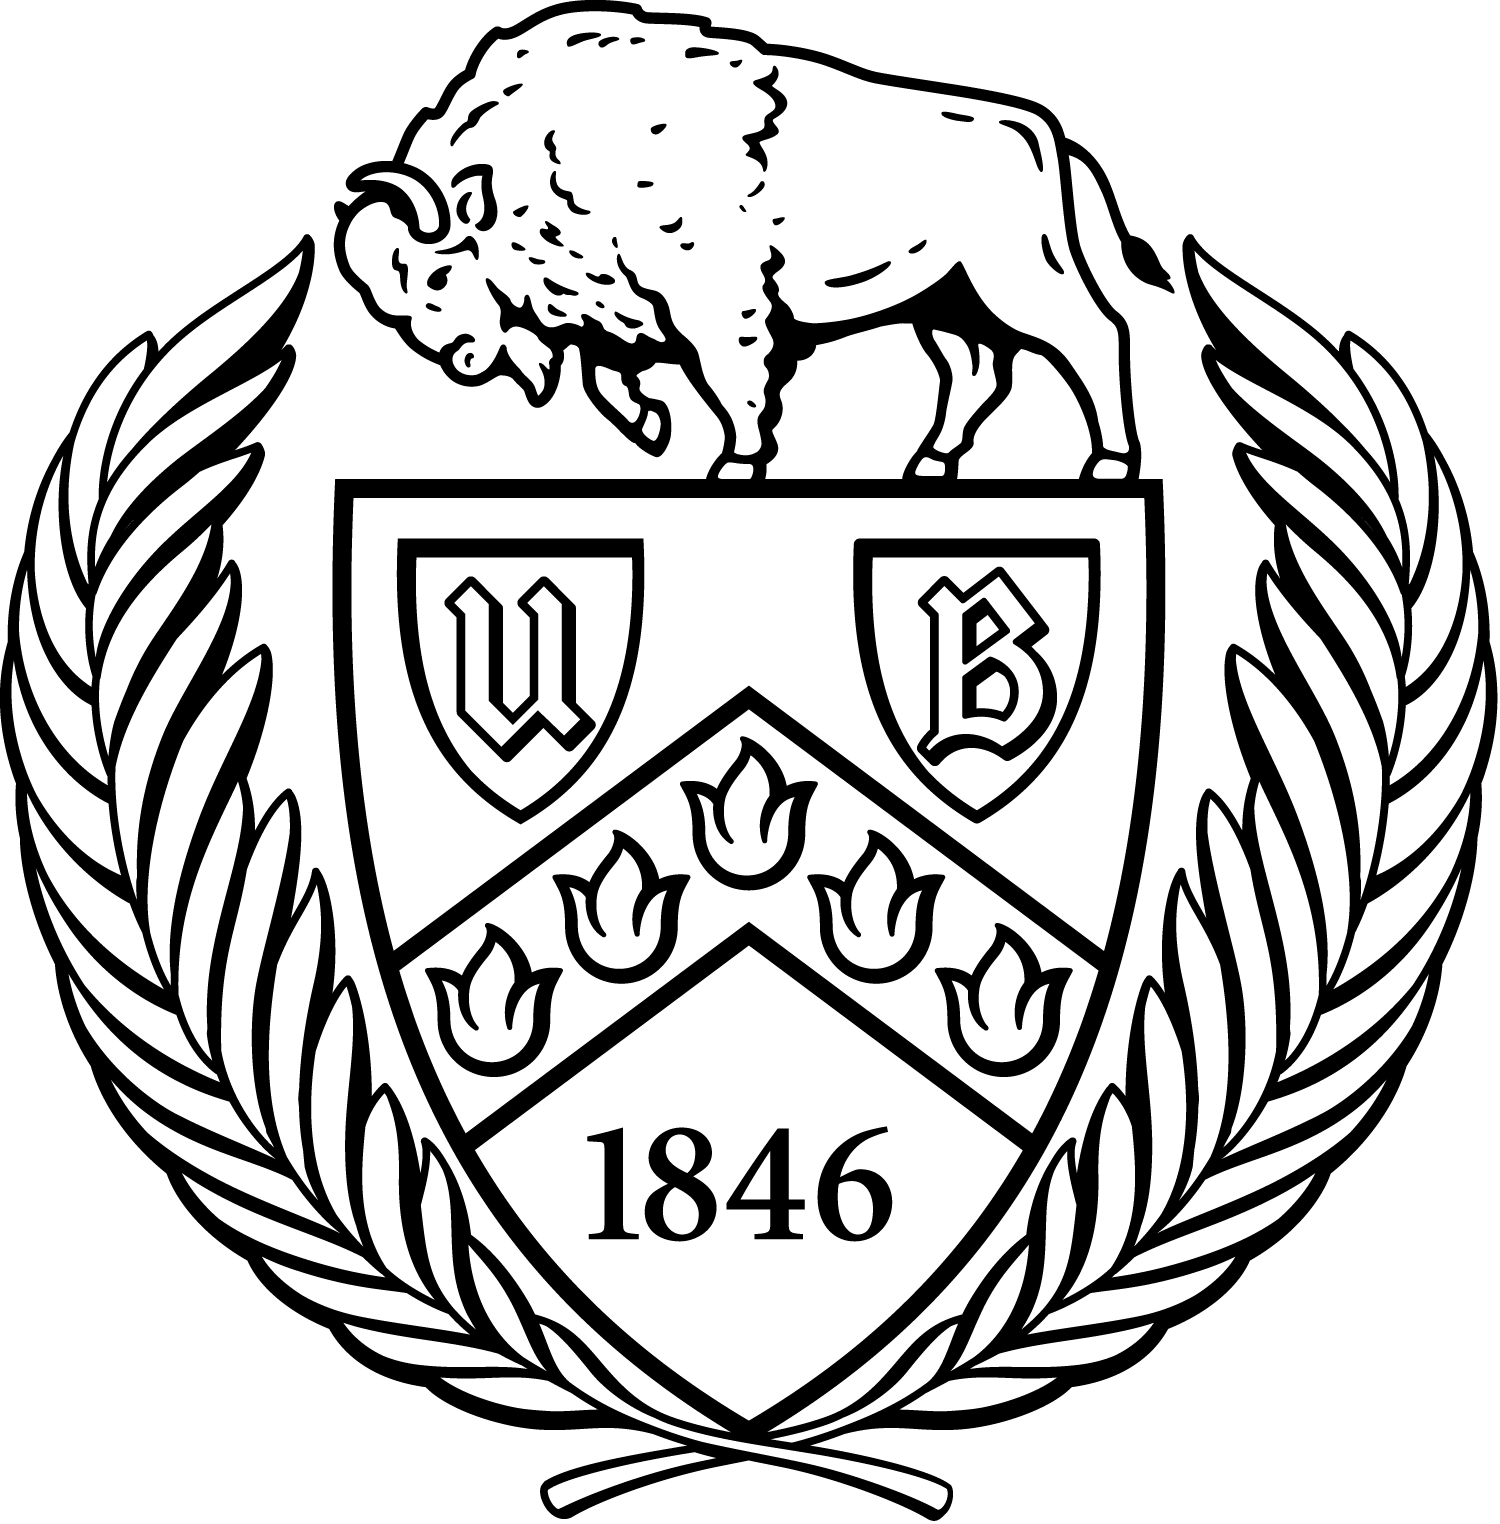
\includegraphics[scale=0.03]{crestUB.png}}

% ------ End Preamble -------


\begin{document}

\begin{frame}
    \maketitle
\end{frame}

\begin{frame}{Table of Contents}
    \tableofcontents
\end{frame}


\begin{frame}{Frame Title}
This is a text in the first frame.
\end{frame}

\section{Section 1}

\begin{frame}{Bullet Lists}

    This is a bullet list, with effects.
    \begin{itemize}\setlength\itemsep{1em}
        \item<1-> Text on slide 1-4
        \item<2-> Text on slide 2-4
        \item<3> Text only on slide 3
        \item<4-> Text on slide 4
    \end{itemize}
    
\end{frame}

\section{Section 2}

\begin{frame}{Blocks for Emphasis}
    \begin{block}{Remark}
        Sample remark
    \end{block}

    \begin{alertblock}{Theorem}        
        Sample theorem in red
    \end{alertblock}
    
    \begin{example}
        Examples are shown in green
    \end{example}
\end{frame}

\begin{frame}{Columns}
    \begin{columns}
        \column{0.5\textwidth}
        First column text
        $$ \sum_{j \in \delta^+(i)} x_{ij} - \sum_{j \in \delta^-(i)} x_{ji} = b_i$$
        
        \begin{itemize}
            \item First item
            \item Second item
        \end{itemize}

        \column{0.5\textwidth}
        Second column text. Second column provides a nice layout
    \end{columns}
\end{frame}

\begin{frame}[t]{Overlay Area}
    %
\documentclass[tikz]{standalone}
\usepackage{tikz}
\usetikzlibrary{positioning, automata, fit, shapes, chains}


\begin{document}
    \begin{tikzpicture}
    \node[state, minimum size = 3pt] (0) {0};
    \node[above right=0.025cm and 0.25cm of 0,text width=1.5cm, inner sep =0.25pt] (obj0) {\tiny$z^* = 8.2$};
    \node[below = 0.005cm of obj0,text width=1.5cm] (sol0) {\tiny$(3.8,3)$};
    \node[right=3cm of 0, text width =1.5cm] {\small UB = 8.2 LB = 0};
    \node[black!0,state, minimum size = 3pt, below left =1cm and 2cm of 0] (1) {1};
    \node[black!0,state, minimum size = 3pt, below right =1cm and 2cm of 0] (2) {2};
    \node[black!0,state, minimum size = 3pt, below left =of 2] (3) {3};
    \node[black!0,state, minimum size = 3pt, below right =of 2] (4) {4};
    \node[black!0,above right=0.001cm and 0.4cm of 4,text width=1.5cm, inner sep =0.25pt] (obj4) {\tiny$z^* = 4$};

    \node[black!0,below = 0.005cm of obj4,text width=1.5cm] (sol4) {\tiny$(4,2)$};
    \node[black!0,state, minimum size = 3pt, below left =of 1] (5) {5};
    \node[black!0,state, minimum size = 3pt, below right =of 1] (6) {6};
    \node[black!0,state, minimum size = 3pt, below left =of 6] (7) {7};
    \node[black!0,state, minimum size = 3pt, below right =of 6] (8) {8};
    \end{tikzpicture}
  
        \begin{tikzpicture}
        \node[state, minimum size = 3pt] (0) {0};
        \node[above right=0.025cm and 0.25cm of 0,text width=1.5cm, inner sep =0.25pt] (obj0) {\tiny$z^* = 8.2$};
        \node[below = 0.005cm of obj0,text width=1.5cm] (sol0) {\tiny$(3.8,3)$};
        \node[right=3cm of 0, text width =1.5cm] {\small UB = 7.6 LB = 0};
        \node[state, minimum size = 3pt, below left =1cm and 2cm of 0] (1) {1};
        \node[above right=0.001cm and 0.4cm of 1,text width=1.5cm, inner sep =0.25pt] (obj1) {\tiny$z^* = 7.4$};
        \node[below = 0.005cm of obj1,text width=1.5cm] (sol1) {\tiny$(3, 2.6)$};
        \node[state, minimum size = 3pt, below right =1cm and 2cm of 0] (2) {2};
        \node[above right=0.001cm and 0.4cm of 2,text width=1.5cm, inner sep =0.25pt] (obj2) {\tiny$z^* = 7.6$};
        \node[below = 0.005cm of obj2,text width=1.5cm] (sol2) {\tiny$(4, 2.9)$};
        \node[black!0,state, minimum size = 3pt, below left =of 2] (3) {3};
        \node[black!0,state, minimum size = 3pt, below right =of 2] (4) {4};
        \node[black!0,above right=0.001cm and 0.4cm of 4,text width=1.5cm, inner sep =0.25pt] (obj4) {\tiny$z^* = 4$};
        \node[black!0, below = 0.005cm of obj4,text width=1.5cm] (sol4) {\tiny$(4,2)$};
        \node[black!0,state, minimum size = 3pt, below left =of 1] (5) {5};
        \node[black!0,state, minimum size = 3pt, below right =of 1] (6) {6};
        \node[black!0,state, minimum size = 3pt, below left =of 6] (7) {7};
        \node[black!0,state, minimum size = 3pt, below right =of 6] (8) {8};
        \path[->]
        (0) edge node [above, sloped] {\tiny$x_1 \leq 3$} (1)
        (0) edge node [above, sloped] {\tiny$x_1 \geq 4$} (2);
        \end{tikzpicture}
  
        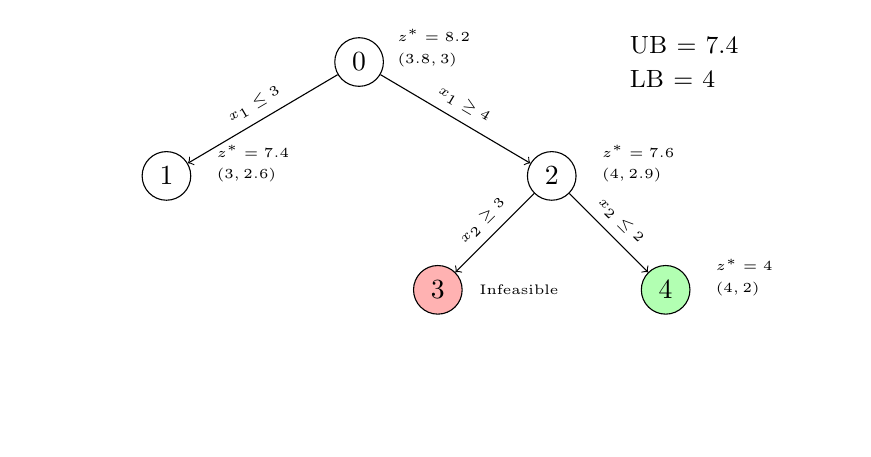
\begin{tikzpicture}
        \node[state, minimum size = 3pt] (0) {0};
        \node[state, minimum size = 3pt, below left =1cm and 2cm of 0] (1) {1};
        \node[state, minimum size = 3pt, below right =1cm and 2cm of 0] (2) {2};
        \node[fill=red!30,state, minimum size = 3pt, below left =of 2] (3) {3};
        \node[fill=green!30,state, minimum size = 3pt, below right =of 2] (4) {4};
        \node[black!0,state, minimum size = 3pt, below left =of 1] (5) {5};
        \node[black!0,state, minimum size = 3pt, below right =of 1] (6) {6};
        \node[black!0,state, minimum size = 3pt, below left =of 6] (7) {7};
        \node[black!0,state, minimum size = 3pt, below right =of 6] (8) {8};
        %---------------------------
        \node[right=3cm of 0, text width =1.5cm] {\small UB = 7.4 LB = 4};
        \node[above right=0.025cm and 0.25cm of 0,text width=1.5cm, inner sep =0.25pt] (obj0) {\tiny$z^* = 8.2$};
        \node[below = 0.005cm of obj0,text width=1.5cm] (sol0) {\tiny$(3.8,3)$};
        \node[above right=0.001cm and 0.4cm of 1,text width=1.5cm, inner sep =0.25pt] (obj1) {\tiny$z^* = 7.4$};
        \node[below = 0.005cm of obj1,text width=1.5cm] (sol1) {\tiny$(3, 2.6)$};
        \node[above right=0.001cm and 0.4cm of 2,text width=1.5cm, inner sep =0.25pt] (obj2) {\tiny$z^* = 7.6$};
        \node[below = 0.005cm of obj2,text width=1.5cm] (sol2) {\tiny$(4, 2.9)$};
        \node[right=0.2cm of 3,text width=1.5cm, inner sep =0.25pt] (obj3) {\tiny Infeasible};
        \node[above right=0.001cm and 0.4cm of 4,text width=1.5cm, inner sep =0.25pt] (obj4) {\tiny$z^* = 4$};
        \node[below = 0.005cm of obj4,text width=1.5cm] (sol4) {\tiny$(4,2)$};
        %--------------------------
        \path[->]
        (2) edge node [above, sloped] {\tiny$x_2 \geq 3$} (3)
        (2) edge node [above, sloped] {\tiny$x_2 \leq 2$} (4)
        (0) edge node [above, sloped] {\tiny$x_1 \leq 3$} (1)
        (0) edge node [above, sloped] {\tiny$x_1 \geq 4$} (2);
        \end{tikzpicture}
    
        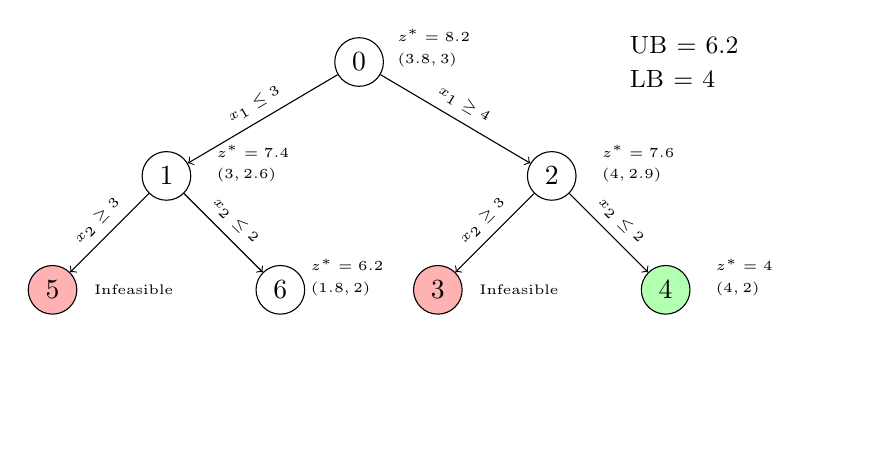
\begin{tikzpicture}
        \node[state, minimum size = 3pt] (0) {0};
        \node[state, minimum size = 3pt, below left =1cm and 2cm of 0] (1) {1};
        \node[state, minimum size = 3pt, below right =1cm and 2cm of 0] (2) {2};
        \node[fill=red!30,state, minimum size = 3pt, below left =of 2] (3) {3};
        \node[fill=green!30,state, minimum size = 3pt, below right =of 2] (4) {4};
        \node[fill=red!30, state, minimum size = 3pt, below left =of 1] (5) {5};
        \node[state, minimum size = 3pt, below right =of 1] (6) {6};
        \node[black!0,state, minimum size = 3pt, below left =of 6] (7) {7};
        \node[black!0,state, minimum size = 3pt, below right =of 6] (8) {8};
        %---------------------------
        \node[right=3cm of 0, text width =1.5cm] {\small UB = 6.2 LB = 4};
        \node[above right=0.025cm and 0.25cm of 0,text width=1.5cm, inner sep =0.25pt] (obj0) {\tiny$z^* = 8.2$};
        \node[below = 0.005cm of obj0,text width=1.5cm] (sol0) {\tiny$(3.8,3)$};
        \node[above right=0.001cm and 0.4cm of 1,text width=1.5cm, inner sep =0.25pt] (obj1) {\tiny$z^* = 7.4$};
        \node[below = 0.005cm of obj1,text width=1.5cm] (sol1) {\tiny$(3, 2.6)$};
        \node[above right=0.001cm and 0.4cm of 2,text width=1.5cm, inner sep =0.25pt] (obj2) {\tiny$z^* = 7.6$};
        \node[below = 0.005cm of obj2,text width=1.5cm] (sol2) {\tiny$(4, 2.9)$};
        \node[right=0.2cm of 3,text width=1.5cm, inner sep =0.25pt] (obj3) {\tiny Infeasible};
        \node[above right=0.001cm and 0.4cm of 4,text width=1.5cm, inner sep =0.25pt] (obj4) {\tiny$z^* = 4$};
        \node[below = 0.005cm of obj4,text width=1.5cm] (sol4) {\tiny$(4,2)$};
        \node[right=0.2cm of 5,text width=1.5cm, inner sep =0.25pt] (obj5) {\tiny Infeasible};
        \node[above right=0.001cm and 0.15cm of 6,text width=1.5cm, inner sep =0.25pt] (obj6) {\tiny$z^* = 6.2$};
        \node[below = 0.005cm of obj6,text width=1.5cm] (sol6) {\tiny$(1.8, 2)$};
        %--------------------------
        \path[->]
        (1) edge node [above, sloped] {\tiny$x_2 \geq 3$} (5)
        (1) edge node [above, sloped] {\tiny$x_2 \leq 2$} (6)
        (2) edge node [above, sloped] {\tiny$x_2 \geq 3$} (3)
        (2) edge node [above, sloped] {\tiny$x_2 \leq 2$} (4)
        (0) edge node [above, sloped] {\tiny$x_1 \leq 3$} (1)
        (0) edge node [above, sloped] {\tiny$x_1 \geq 4$} (2);
        \end{tikzpicture}
    
        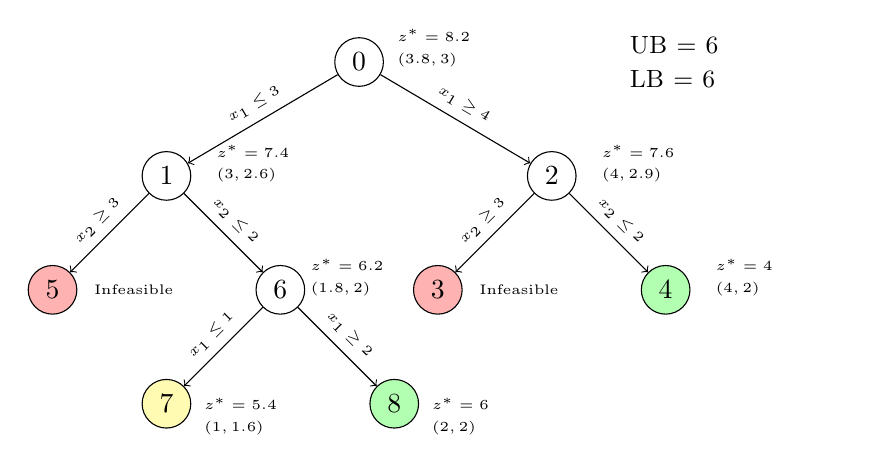
\begin{tikzpicture}
        \node[state, minimum size = 3pt] (0) {0};
        \node[state, minimum size = 3pt, below left =1cm and 2cm of 0] (1) {1};
        \node[state, minimum size = 3pt, below right =1cm and 2cm of 0] (2) {2};
        \node[fill=red!30,state, minimum size = 3pt, below left =of 2] (3) {3};
        \node[fill=green!30,state, minimum size = 3pt, below right =of 2] (4) {4};
        \node[fill=red!30, state, minimum size = 3pt, below left =of 1] (5) {5};
        \node[state, minimum size = 3pt, below right =of 1] (6) {6};
        \node[fill=yellow!30, state, minimum size = 3pt, below left =of 6] (7) {7};
        \node[fill=green!30,state, minimum size = 3pt, below right =of 6] (8) {8};
        %---------------------------
        \node[right=3cm of 0, text width =1.5cm] {\small UB = 6 LB = 6};
        \node[above right=0.025cm and 0.25cm of 0,text width=1.5cm, inner sep =0.25pt] (obj0) {\tiny$z^* = 8.2$};
        \node[below = 0.005cm of obj0,text width=1.5cm] (sol0) {\tiny$(3.8,3)$};
        \node[above right=0.001cm and 0.4cm of 1,text width=1.5cm, inner sep =0.25pt] (obj1) {\tiny$z^* = 7.4$};
        \node[below = 0.005cm of obj1,text width=1.5cm] (sol1) {\tiny$(3, 2.6)$};
        \node[above right=0.001cm and 0.4cm of 2,text width=1.5cm, inner sep =0.25pt] (obj2) {\tiny$z^* = 7.6$};
        \node[below = 0.005cm of obj2,text width=1.5cm] (sol2) {\tiny$(4, 2.9)$};
        \node[right=0.2cm of 3,text width=1.5cm, inner sep =0.25pt] (obj3) {\tiny Infeasible};
        \node[above right=0.001cm and 0.4cm of 4,text width=1.5cm, inner sep =0.25pt] (obj4) {\tiny$z^* = 4$};
        \node[below = 0.005cm of obj4,text width=1.5cm] (sol4) {\tiny$(4,2)$};
        \node[right=0.2cm of 5,text width=1.5cm, inner sep =0.25pt] (obj5) {\tiny Infeasible};
        \node[above right=0.001cm and 0.15cm of 6,text width=1.5cm, inner sep =0.25pt] (obj6) {\tiny$z^* = 6.2$};
        \node[below = 0.005cm of obj6,text width=1.5cm] (sol6) {\tiny$(1.8, 2)$};
        \node[right= 0.15cm of 7,text width=1.5cm, inner sep =0.25pt] (obj7) {\tiny$z^* = 5.4$};
        \node[below = 0.005cm of obj7,text width=1.5cm] (sol7) {\tiny$(1, 1.6)$};
        \node[right= 0.15cm of 8,text width=1.5cm, inner sep =0.25pt] (obj8) {\tiny$z^* = 6$};
        \node[below = 0.005cm of obj8,text width=1.5cm] (sol8) {\tiny$(2,2)$};
        %--------------------------
        \path[->]
        (6) edge node [above, sloped] {\tiny$x_1 \leq 1$} (7)
        (6) edge node [above, sloped] {\tiny$x_1 \geq2$} (8)
        (1) edge node [above, sloped] {\tiny$x_2 \geq 3$} (5)
        (1) edge node [above, sloped] {\tiny$x_2 \leq 2$} (6)
        (2) edge node [above, sloped] {\tiny$x_2 \geq 3$} (3)
        (2) edge node [above, sloped] {\tiny$x_2 \leq 2$} (4)
        (0) edge node [above, sloped] {\tiny$x_1 \leq 3$} (1)
        (0) edge node [above, sloped] {\tiny$x_1 \geq 4$} (2);
        \end{tikzpicture}
\end{document}
    \begin{itemize}
        \item Use \texttt{overlayarea} environment in order to sequence images without them ``dancing'' on the slide
    \end{itemize}
    \begin{overlayarea}{\textwidth}{4cm}
        \only<1>{
            \begin{center}
                \includestandalone[mode=image, page=1]{img/standalone}
            \end{center}
        }
        \only<2>{
            \begin{center}
                \includestandalone[mode=image, page=2]{img/standalone}
            \end{center}
        }
        \only<3>{
            \begin{center}
                \includestandalone[mode=image, page=3]{img/standalone}
            \end{center}
        }
        \only<4>{
            \begin{center}
                \includestandalone[mode=image, page=4]{img/standalone}
            \end{center}
        }
        \only<5>{
            \begin{center}
                \includestandalone[mode=image, page=5]{img/standalone}
            \end{center}
        }
    \end{overlayarea}
\end{frame} 

\end{document}